% Options for packages loaded elsewhere
\PassOptionsToPackage{unicode}{hyperref}
\PassOptionsToPackage{hyphens}{url}
%
\documentclass[
  english,
  man,floatsintext]{apa6}
\usepackage{lmodern}
\usepackage{amssymb,amsmath}
\usepackage{ifxetex,ifluatex}
\ifnum 0\ifxetex 1\fi\ifluatex 1\fi=0 % if pdftex
  \usepackage[T1]{fontenc}
  \usepackage[utf8]{inputenc}
  \usepackage{textcomp} % provide euro and other symbols
\else % if luatex or xetex
  \usepackage{unicode-math}
  \defaultfontfeatures{Scale=MatchLowercase}
  \defaultfontfeatures[\rmfamily]{Ligatures=TeX,Scale=1}
\fi
% Use upquote if available, for straight quotes in verbatim environments
\IfFileExists{upquote.sty}{\usepackage{upquote}}{}
\IfFileExists{microtype.sty}{% use microtype if available
  \usepackage[]{microtype}
  \UseMicrotypeSet[protrusion]{basicmath} % disable protrusion for tt fonts
}{}
\makeatletter
\@ifundefined{KOMAClassName}{% if non-KOMA class
  \IfFileExists{parskip.sty}{%
    \usepackage{parskip}
  }{% else
    \setlength{\parindent}{0pt}
    \setlength{\parskip}{6pt plus 2pt minus 1pt}}
}{% if KOMA class
  \KOMAoptions{parskip=half}}
\makeatother
\usepackage{xcolor}
\IfFileExists{xurl.sty}{\usepackage{xurl}}{} % add URL line breaks if available
\IfFileExists{bookmark.sty}{\usepackage{bookmark}}{\usepackage{hyperref}}
\hypersetup{
  pdftitle={The title},
  pdfauthor={First Author1 \& Ernst-August Doelle1,2},
  pdflang={en-EN},
  pdfkeywords={keywords},
  hidelinks,
  pdfcreator={LaTeX via pandoc}}
\urlstyle{same} % disable monospaced font for URLs
\usepackage{graphicx}
\makeatletter
\def\maxwidth{\ifdim\Gin@nat@width>\linewidth\linewidth\else\Gin@nat@width\fi}
\def\maxheight{\ifdim\Gin@nat@height>\textheight\textheight\else\Gin@nat@height\fi}
\makeatother
% Scale images if necessary, so that they will not overflow the page
% margins by default, and it is still possible to overwrite the defaults
% using explicit options in \includegraphics[width, height, ...]{}
\setkeys{Gin}{width=\maxwidth,height=\maxheight,keepaspectratio}
% Set default figure placement to htbp
\makeatletter
\def\fps@figure{htbp}
\makeatother
\setlength{\emergencystretch}{3em} % prevent overfull lines
\providecommand{\tightlist}{%
  \setlength{\itemsep}{0pt}\setlength{\parskip}{0pt}}
\setcounter{secnumdepth}{-\maxdimen} % remove section numbering
% Make \paragraph and \subparagraph free-standing
\ifx\paragraph\undefined\else
  \let\oldparagraph\paragraph
  \renewcommand{\paragraph}[1]{\oldparagraph{#1}\mbox{}}
\fi
\ifx\subparagraph\undefined\else
  \let\oldsubparagraph\subparagraph
  \renewcommand{\subparagraph}[1]{\oldsubparagraph{#1}\mbox{}}
\fi
% Manuscript styling
\usepackage{upgreek}
\captionsetup{font=singlespacing,justification=justified}

% Table formatting
\usepackage{longtable}
\usepackage{lscape}
% \usepackage[counterclockwise]{rotating}   % Landscape page setup for large tables
\usepackage{multirow}		% Table styling
\usepackage{tabularx}		% Control Column width
\usepackage[flushleft]{threeparttable}	% Allows for three part tables with a specified notes section
\usepackage{threeparttablex}            % Lets threeparttable work with longtable

% Create new environments so endfloat can handle them
% \newenvironment{ltable}
%   {\begin{landscape}\begin{center}\begin{threeparttable}}
%   {\end{threeparttable}\end{center}\end{landscape}}
\newenvironment{lltable}{\begin{landscape}\begin{center}\begin{ThreePartTable}}{\end{ThreePartTable}\end{center}\end{landscape}}

% Enables adjusting longtable caption width to table width
% Solution found at http://golatex.de/longtable-mit-caption-so-breit-wie-die-tabelle-t15767.html
\makeatletter
\newcommand\LastLTentrywidth{1em}
\newlength\longtablewidth
\setlength{\longtablewidth}{1in}
\newcommand{\getlongtablewidth}{\begingroup \ifcsname LT@\roman{LT@tables}\endcsname \global\longtablewidth=0pt \renewcommand{\LT@entry}[2]{\global\advance\longtablewidth by ##2\relax\gdef\LastLTentrywidth{##2}}\@nameuse{LT@\roman{LT@tables}} \fi \endgroup}

% \setlength{\parindent}{0.5in}
% \setlength{\parskip}{0pt plus 0pt minus 0pt}

% \usepackage{etoolbox}
\makeatletter
\patchcmd{\HyOrg@maketitle}
  {\section{\normalfont\normalsize\abstractname}}
  {\section*{\normalfont\normalsize\abstractname}}
  {}{\typeout{Failed to patch abstract.}}
\patchcmd{\HyOrg@maketitle}
  {\section{\protect\normalfont{\@title}}}
  {\section*{\protect\normalfont{\@title}}}
  {}{\typeout{Failed to patch title.}}
\makeatother
\shorttitle{Title}
\keywords{keywords\newline\indent Word count: X}
\usepackage{lineno}

\linenumbers
\usepackage{csquotes}
\ifxetex
  % Load polyglossia as late as possible: uses bidi with RTL langages (e.g. Hebrew, Arabic)
  \usepackage{polyglossia}
  \setmainlanguage[]{english}
\else
  \usepackage[shorthands=off,main=english]{babel}
\fi
\newlength{\cslhangindent}
\setlength{\cslhangindent}{1.5em}
\newenvironment{cslreferences}%
  {\setlength{\parindent}{0pt}%
  \everypar{\setlength{\hangindent}{\cslhangindent}}\ignorespaces}%
  {\par}

\title{The title}
\author{First Author\textsuperscript{1} \& Ernst-August Doelle\textsuperscript{1,2}}
\date{}


\authornote{

Add complete departmental affiliations for each author here. Each new line herein must be indented, like this line.

Enter author note here.

The authors made the following contributions. First Author: Conceptualization, Writing - Original Draft Preparation, Writing - Review \& Editing; Ernst-August Doelle: Writing - Review \& Editing.

Correspondence concerning this article should be addressed to First Author, Postal address. E-mail: \href{mailto:my@email.com}{\nolinkurl{my@email.com}}

}

\affiliation{\vspace{0.5cm}\textsuperscript{1} Wilhelm-Wundt-University\\\textsuperscript{2} Konstanz Business School}

\abstract{
One or two sentences providing a \textbf{basic introduction} to the field, comprehensible to a scientist in any discipline.

Two to three sentences of \textbf{more detailed background}, comprehensible to scientists in related disciplines.

One sentence clearly stating the \textbf{general problem} being addressed by this particular study.

One sentence summarizing the main result (with the words ``\textbf{here we show}'' or their equivalent).

Two or three sentences explaining what the \textbf{main result} reveals in direct comparison to what was thought to be the case previously, or how the main result adds to previous knowledge.

One or two sentences to put the results into a more \textbf{general context}.

Two or three sentences to provide a \textbf{broader perspective}, readily comprehensible to a scientist in any discipline.
}



\begin{document}
\maketitle

This text is for the body of the introduction. This is how you \textbf{bold} text. This is \emph{italics}. Lorem ipsum dolor sit amet, consectetur adipiscing elit. Integer fringilla orci odio, eget venenatis diam aliquet nec.\footnote{This is a footnote.} Vivamus sodales aliquam tortor ac scelerisque. Nullam laoreet est id dolor rhoncus bibendum. Etiam eleifend, tortor vel euismod ullamcorper, nunc enim lacinia eros, at semper nulla arcu eget est. Pellentesque dapibus euismod sem, sed sollicitudin nisi blandit ac. Quisque dapibus lorem id felis cursus, id placerat magna dapibus. Sed id nibh dictum, tristique nulla non, tempor ipsum.\footnote{This is another footnote.}

\hypertarget{first-level-header}{%
\section{First level header}\label{first-level-header}}

In sit amet arcu congue, elementum tellus nec, pellentesque libero. Nulla facilisi. Aenean ornare nisi eget lacus pulvinar, eget imperdiet massa dignissim. Aliquam scelerisque ut libero sed condimentum. Sed ut consectetur justo.

\hypertarget{second-level-header}{%
\subsection{Second level header}\label{second-level-header}}

Quisque dapibus sem non fringilla volutpat. Sed finibus magna et eros pharetra posuere. Nunc id elit metus. Mauris quis malesuada massa. Fusce et auctor felis. Aenean id sem ex. Nulla viverra leo in quam cursus auctor. Nullam rutrum erat quis lobortis ullamcorper.

\hypertarget{third-level-header}{%
\subsubsection{Third level header}\label{third-level-header}}

Quisque dapibus sem non fringilla volutpat. Sed finibus magna et eros pharetra posuere. Nunc id elit metus. Mauris quis malesuada massa. Fusce et auctor felis. Aenean id sem ex. Nulla viverra leo in quam cursus auctor. Nullam rutrum erat quis lobortis ullamcorper.

\hypertarget{citations}{%
\section{Citations}\label{citations}}

Citations are similar to Latex. Place bibliographic entries in a .bib file, then link to the .bib file in the YAML above. This example uses \texttt{example.bib}. Use a reference manager like Zotero to export bib files for collections of manuscripts, or write them by hand, or copy and paste from google scholar.

An example of citing a paper with author year in parentheses (Crump \& Logan, 2010). Separate citation keys with semicolons to add multiple citations (Crump \& Logan, 2010; Jamieson, Hannah, \& Crump, 2010).

To cite the author alone with year in parentheses use Crump and Logan (2010). To cite year only, use (2010).

To add a prefix to the citation (see also, Crump \& Logan, 2010). To add a postfix (see also, Crump \& Logan, 2010, for a review)

\hypertarget{equations}{%
\section{Equations}\label{equations}}

Use Latex syntax for math equations by placing formulas between dollar signs.

\(a^2 + b^2 = c^2\)

You should see a preview of the equation in RStudio if you hover over the equation.

Include equations inside Latex style syntax for cross-referencing. Note, this also illustrates that latex syntax can be written directly, and will be treated as Latex for compiling the output.

\begin{equation}
a_i = (\frac{\sum_{j=1}^{j=n}p_j \times M_{ij}}{\sqrt{\sum_{j=1}^{j=n}p_j^2}\sqrt{\sum_{j=1}^{j=n}M_{ij}^2}})^{tau}
\label{eq:activation}
\end{equation}

Cross reference the equation like this, see Equation~\eqref{eq:activation}.

\hypertarget{external-images}{%
\section{External images}\label{external-images}}

Using \texttt{knitr::include\_graphics()} is a versatile method for inserting external images. The file path is relative to the folder containing the .Rmd file for the manuscript. In this case, the \texttt{logo.png} file is in the same folder as \texttt{manuscript.Rmd}, so we simply locate the file directly.

\begin{figure}
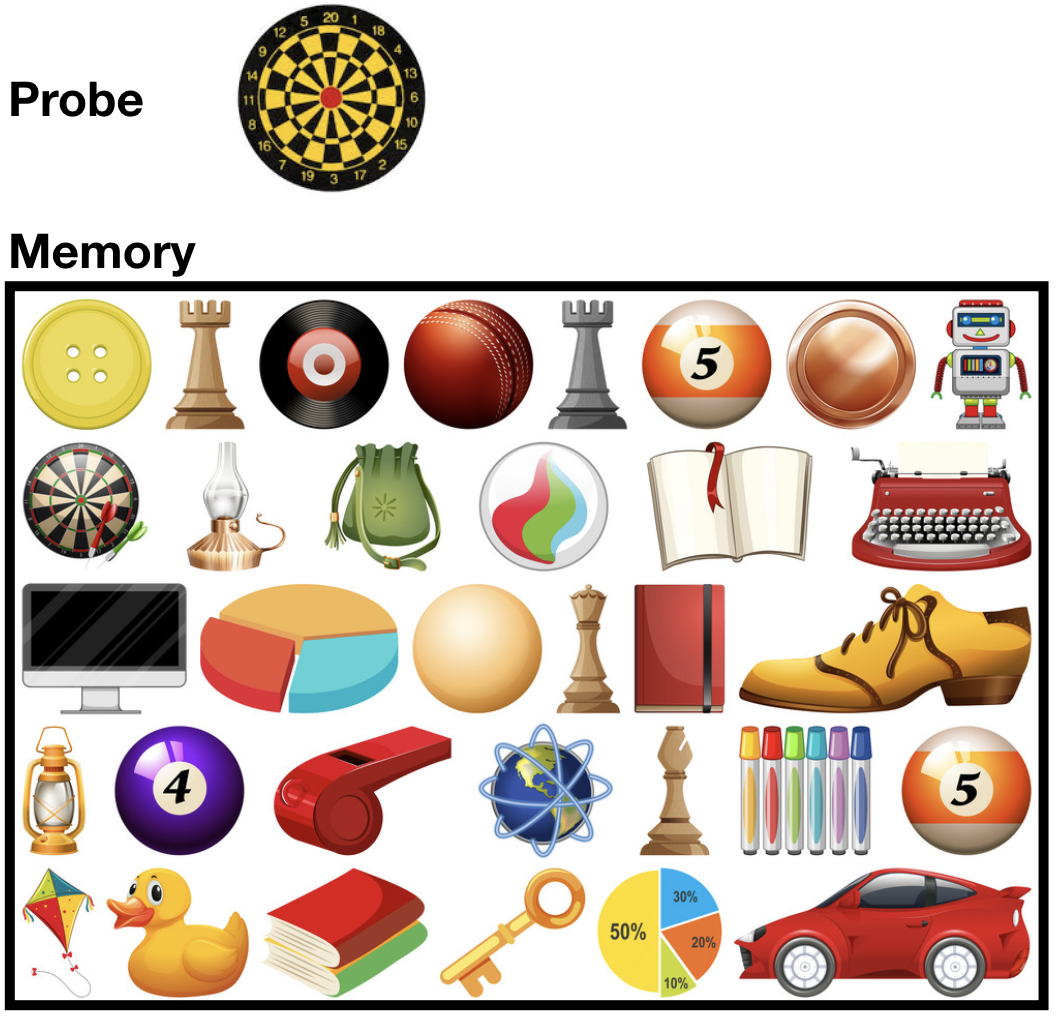
\includegraphics[width=0.5\linewidth]{external_image} \caption{An example external image.}\label{fig:vertical}
\end{figure}

The name for the codechunk above is \texttt{vertical}, which can later be used as a cross-reference to figure, see Figure \ref{fig:vertical}.

\hypertarget{experiment-1}{%
\section{Experiment 1}\label{experiment-1}}

\hypertarget{methods}{%
\subsection{Methods}\label{methods}}

We report how we determined our sample size, all data exclusions (if any), all manipulations, and all measures in the study.

\hypertarget{participants}{%
\subsubsection{Participants}\label{participants}}

\hypertarget{material}{%
\subsubsection{Material}\label{material}}

\hypertarget{procedure}{%
\subsubsection{Procedure}\label{procedure}}

\hypertarget{data-analysis}{%
\subsubsection{Data analysis}\label{data-analysis}}

We used R (Version 3.6.0; R Core Team, 2019) and the R-packages \emph{dplyr} (Version 1.0.1; Wickham et al., 2019), \emph{ggplot2} (Version 3.2.0; Wickham, 2016), \emph{kableExtra} (Version 1.1.0; Zhu, 2019), \emph{nomnoml} (Version 0.1.0; Luraschi, 2019), \emph{papaja} (Version 0.1.0.9997; Aust \& Barth, 2018), \emph{tidyr} (Version 1.1.1; Wickham \& Henry, 2019), and \emph{verticaltutorial} (Version 0.0.0.9000; Crump, n.d.) for all our analyses.

\hypertarget{results}{%
\subsection{Results}\label{results}}

Content stored in R variables can be injected into the document. However, the R variables must be defined before they can be inserted. For example, the following code chunk assigns a values of 1 to a variable x.

Now, the content of this variable can be reported using an inline r code chunk as follows, the value of x is 1.

\begin{table}

\caption{\label{tab:meanstable}Mean Reaction Times and Standard Errors of the Mean for Experiment 3}
\centering
\begin{tabular}[t]{lrrrr}
\toprule
\multicolumn{1}{c}{ } & \multicolumn{2}{c}{Congruent} & \multicolumn{2}{c}{Incongruent} \\
\cmidrule(l{3pt}r{3pt}){2-3} \cmidrule(l{3pt}r{3pt}){4-5}
posture & RT & SEM & RT & SEM\\
\midrule
Sit & 822 & 17 & 941 & 18\\
Stand & 808 & 15 & 904 & 15\\
\bottomrule
\end{tabular}
\end{table}

\begin{figure}
\centering
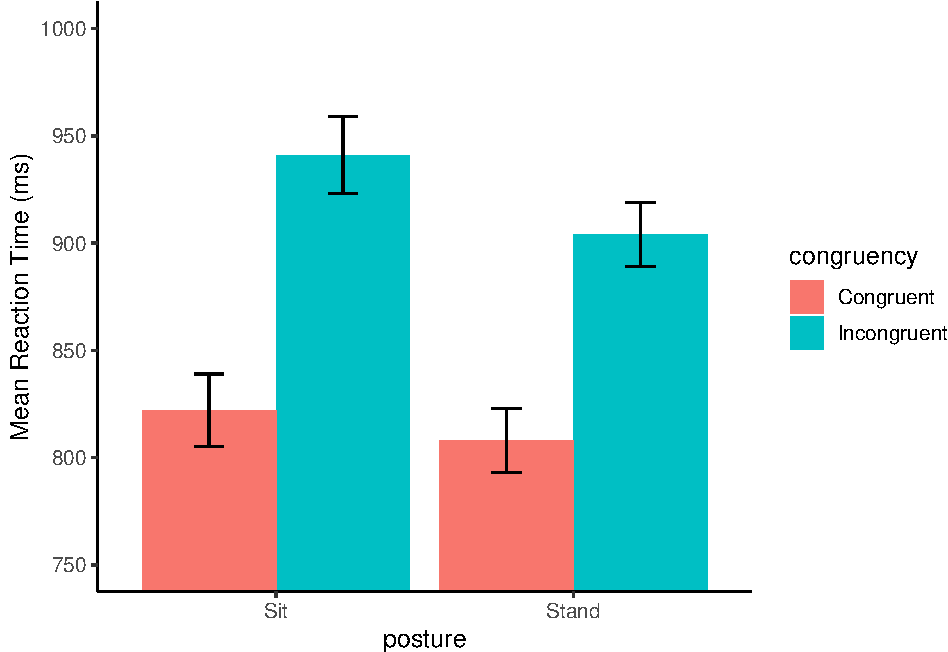
\includegraphics{/Users/mattcrump/Github/verticaltutorial/docs/manuscript/manuscript_files/figure-latex/stroopfig-1.pdf}
\caption{\label{fig:stroopfig}Mean reaction times wth standard error bars as a function of Posture and Congruency for Experiment 3}
\end{figure}

\begin{table}[tbp]

\begin{center}
\begin{threeparttable}

\caption{\label{tab:aovtable}ANOVA table for Experiment 3}

\begin{tabular}{lllllll}
\toprule
Effect & \multicolumn{1}{c}{$F$} & \multicolumn{1}{c}{$\mathit{df}_1$} & \multicolumn{1}{c}{$\mathit{df}_2$} & \multicolumn{1}{c}{$\mathit{MSE}$} & \multicolumn{1}{c}{$p$} & \multicolumn{1}{c}{$\hat{\eta}^2_G$}\\
\midrule
Posture & 7.33 & 1 & 49 & 4,407.09 & .009 & .012\\
Congruency & 342.45 & 1 & 49 & 1,684.39 & < .001 & .182\\
Posture $\times$ Congruency & 8.96 & 1 & 49 & 731.82 & .004 & .003\\
\bottomrule
\end{tabular}

\end{threeparttable}
\end{center}

\end{table}

Below are examples of writing the results using two methods. The first method is to report all of the values by hand. The second method is to embed the results of R variables into the reporting using papaja. Both results sections appear similar in the .pdf, so look at the .rmd file for this example to see how to use papaja.

\hypertarget{by-hand-reporting}{%
\subsection{By hand reporting}\label{by-hand-reporting}}

Mean reaction times for each subject in each condition to a 2 (Congruency: congruent vs.~incongruent) x 2 (Posture: Standing vs.~Sitting) were submitted to a repeated measures ANOVA. Mean RTs in each condition are displayed in Table \ref{tab:meanstable}, and in Figure \ref{fig:stroopfig}. The full ANOVA table is reported in Table \ref{tab:aovtable}.

There was a main effect of Congruency, F (1, 49) = 342.45, MSE = 1684.39, p \textless{} 0.001. Mean reaction times were slower for incongruent (922 ms) than congruent groups (815 ms).

There main effect of Posture was significant, F (1, 49) = 7.33, MSE = 4407.09, p =.009. Mean reaction times were slower for sitting (881 ms) than standing groups (855 ms).

The two-way interaction between Congruency and Posture was significant, F (1, 49) = 8.96, MSE = 731.82, p \textless{} 0.004. The Stroop effect was 23 ms smaller in the standing than sitting conditions.

\hypertarget{papaja-reporting}{%
\subsection{papaja reporting}\label{papaja-reporting}}

There was a main effect of Congruency, \(F(1, 49) = 342.45\), \(\mathit{MSE} = 1,684.39\), \(p < .001\), \(\hat{\eta}^2_G = .182\). Mean reaction times were slower for incongruent (922 ms) than congruent groups (815 ms).

There main effect of Posture was significant, \(F(1, 49) = 7.33\), \(\mathit{MSE} = 4,407.09\), \(p = .009\), \(\hat{\eta}^2_G = .012\). Mean reaction times were slower for sitting (881 ms) than standing groups (855 ms).

The two-way interaction between Congruency and Posture was significant, \(F(1, 49) = 8.96\), \(\mathit{MSE} = 731.82\), \(p = .004\), \(\hat{\eta}^2_G = .003\). The Stroop effect was 23 ms smaller in the standing than sitting conditions.

Note, I used the \texttt{apa\_print()} function to automate reporting of the ANOVA statistics, however in this example I did not automate reporting of the means. This would be possible by separately computing the means of interest, and then reporting them using inline r chunks.

\hypertarget{discussion}{%
\subsection{Discussion}\label{discussion}}

\hypertarget{general-discussion}{%
\section{General Discussion}\label{general-discussion}}

\newpage

\hypertarget{references}{%
\section{References}\label{references}}

\begingroup
\setlength{\parindent}{-0.5in}
\setlength{\leftskip}{0.5in}

\hypertarget{refs}{}
\begin{cslreferences}
\leavevmode\hypertarget{ref-R-papaja}{}%
Aust, F., \& Barth, M. (2018). \emph{papaja: Create APA manuscripts with R Markdown}. Retrieved from \url{https://github.com/crsh/papaja}

\leavevmode\hypertarget{ref-R-verticaltutorial}{}%
Crump, M. J. C. (n.d.). \emph{Verticaltutorial: What the package does (one line, title case)}.

\leavevmode\hypertarget{ref-crumpContextualControlTaskset2010}{}%
Crump, M. J. C., \& Logan, G. D. (2010). Contextual control over task-set retrieval. \emph{Attention, Perception \& Psychophysics}, \emph{72}(8), 2047--2053. \url{https://doi.org/10.3758/APP.72.8.2047}

\leavevmode\hypertarget{ref-jamiesonMemorybasedAccountRetrospective2010}{}%
Jamieson, R. K., Hannah, S. D., \& Crump, M. J. C. (2010). A memory-based account of retrospective revaluation. \emph{Canadian Journal of Experimental Psychology}, \emph{64}(3), 153--164. \url{https://doi.org/10.1037/a0020886}

\leavevmode\hypertarget{ref-R-nomnoml}{}%
Luraschi, J. (2019). \emph{Nomnoml: Sassy 'uml' diagrams}. Retrieved from \url{https://CRAN.R-project.org/package=nomnoml}

\leavevmode\hypertarget{ref-R-base}{}%
R Core Team. (2019). \emph{R: A language and environment for statistical computing}. Vienna, Austria: R Foundation for Statistical Computing. Retrieved from \url{https://www.R-project.org/}

\leavevmode\hypertarget{ref-R-ggplot2}{}%
Wickham, H. (2016). \emph{Ggplot2: Elegant graphics for data analysis}. Springer-Verlag New York. Retrieved from \url{https://ggplot2.tidyverse.org}

\leavevmode\hypertarget{ref-R-dplyr}{}%
Wickham, H., François, R., Henry, L., \& Müller, K. (2019). \emph{Dplyr: A grammar of data manipulation}. Retrieved from \url{https://CRAN.R-project.org/package=dplyr}

\leavevmode\hypertarget{ref-R-tidyr}{}%
Wickham, H., \& Henry, L. (2019). \emph{Tidyr: Tidy messy data}. Retrieved from \url{https://CRAN.R-project.org/package=tidyr}

\leavevmode\hypertarget{ref-R-kableExtra}{}%
Zhu, H. (2019). \emph{KableExtra: Construct complex table with 'kable' and pipe syntax}. Retrieved from \url{https://CRAN.R-project.org/package=kableExtra}
\end{cslreferences}

\endgroup


\end{document}
